


\part{Extendiendo el Simulador simusched}

\section{Ejercicio 3}

Completamos la implementaci\'on del scheduler \rr implementando los \textit{TODOs} de la clase SchedRR.

Este scheduler recibe un \quantum y permite a cada tarea ejecutar como m\'aximo ese tiempo. Una vez finalizado ese tiempo contin\'ua con la siguiente tarea lista para ejecutar.

Para implementar \rr usamos una Cola para ir encolando los procesos que estan listos para ser ejecutados, un n\'umero para acumular la \quota (tiempo que el programa corriente esta ejecutando) y otro n\'umero para guardar el \quantum pasado por par\'ametro.

Ver resoluci\'on completa en los archivos \verb|sched_rr.cpp| y \verb|sched_rr.h|.

\section{Ejercicio 4}

Realizamos dos lotes de prueba para observar el comportamiento del scheduler \rr. 

Para tal fin creamos el tipo de tarea TaskCPUIOCPU que recibe 3 parametros:

\begin{mydescription}{m}
 \item[n] Tiempo de ejecuci\'on de CPU en ciclos de reloj
 \item[i] Tiempo de ejecuci\'on de IO en ciclos de reloj
 \item[m] Tiempo de ejecuci\'on de CPU en ciclos de reloj
\end{mydescription}

Esta tarea ejecuta en el CPU (n) se bloquea por (i) y luego sigue ejecutando (m).

\subsection{Lote 1}

Creamos el siguiente grupo de tareas en \verb|ejercicio4_1.tsk|

\begin{framed}
\begin{verbatim}
# FILE ejercicio4_1.tsk
*2 TaskCPU 30
TaskCPUIOCPU 10 20 10
\end{verbatim}
\end{framed}

Luego ejecutamos Simusched con los siguientes parametros:

\begin{framed}
\begin{verbatim}
./simusched ejercicio4_1.tsk 1 SchedRR 3 | python graphsched.py > ejercicio4_1.png
\end{verbatim}
\end{framed}

\begin{figure}[h!]
  \caption{Dos tareas de uso intensivo de CPU y una tarea de tipo TaskCPUIOCPU.}
  \centering
    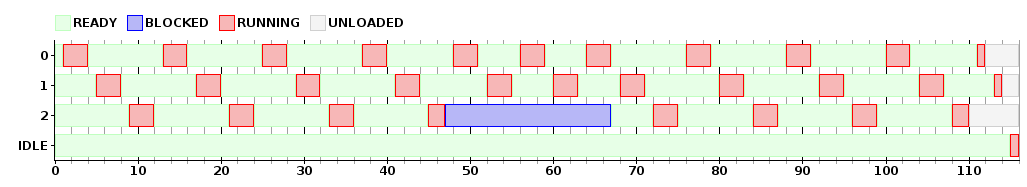
\includegraphics[width=1\textwidth]{img/ejercicio4_1.png}
\end{figure}

Se puede ver en el gr\'afico que se van alternando los 3 procesos con un quantum de 3 unidades hasta que el proceso (2) se bloquea. Mientras el proceso (2) est\'a bloqueado se puede ver que los otros dos procesos van altenando su ejecuci\'on. Hasta que el proceso (2) se desbloquea y nuevamente se vuelven a alternar los 3 procesos.

\subsection{Lote 2}

Utilizamos nuevamente la tarea que creamos anteriormente TaskCPUIOCPU.

Creamos un nuevo lote de tareas en el archivo \verb|ejercicio4_2.tsk|

\begin{framed}
\begin{verbatim}
# FILE ejercicio4_2.tsk
TaskCPUIOCPU 10 20 10
@3
TaskCPUIOCPU 15 20 5
@10
TaskCPU 10
\end{verbatim}
\end{framed}

Luego ejecutamos Simusched con los siguientes parametros:

\begin{framed}
\begin{verbatim}
./simusched ejercicio4_2.tsk 1 SchedRR 4 | python graphsched.py > ejercicio4_2.png
\end{verbatim}
\end{framed}

\begin{figure}[h!]
  \caption{Dos tareas de tipo TaskCPUIOCPU y una tarea de uso intensivo de CPU.}
  \centering
    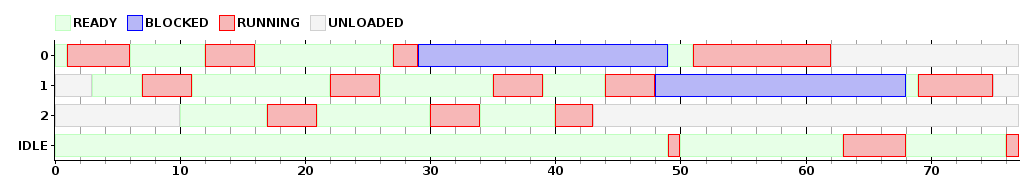
\includegraphics[width=1\textwidth]{img/ejercicio4_2.png}
\end{figure}

Se ve en el gr\'afico que se carga la tarea 0 y se comienza a ejecutar por el quantum de 4.

Luego, cuando la tarea 0 finaliza, la tarea 1 ya est\'a en la cola de listos, por lo que comienza a ejecutarse la tarea 1 hasta finalizar su quantum.

Para ese momento las tareas 0 y 2 est\'an en la cola de listos, por lo que comienza a ejecutar la 0 que estaba en primer lugar.

Despu\'es de eso las tres tareas ya se encuentran cargadas y se van ejecutando hasta finalizar su quantum hasta que el ciclo 29 la tarea 0 se bloquea.

Por lo que siguen ejecutando las tareas 1 y 2 hasta que el el ciclo 43 la tarea 2 finaliza, y en el ciclo 48 la tarea 1 se bloquea, por lo que el procesador queda ocioso.

En el ciclo 49 la tarea 0 finaliza su entrada/salida, por lo que contin\'ua su ejecuci\'on. 

En el ciclo 62 la tarea 0 finaliza y el procesador queda nuevamente ocioso.

En el ciclo 68 la tarea 1 finaliza su entrada/salida y ejecuta hasta finalizar.


\section{Ejercicio 5}

Completamos la implementaci\'on del scheduler \mfq implementando los \textit{TODOs} de la clase SchedMFQ. Este scheduler utiliza n colas con \rr, y recibe como parametro el \quantum de cada una de las colas.

Para implementar \mfq usamos:

\begin{itemize}
 \item una lista de Colas tan larga como la cantidad de quantums pasados como par\'ametro.
 \item una lista con los \quantums de cada cola.
 \item una diccionario para mantener la pioridad asignada a cada proceso.
 \item una n\'umero para acumular la \quota del proceso corriente
\end{itemize}

Ver resoluci\'on completa en los archivos \verb|sched_mfq.cpp| y \verb|sched_mfq.h|.
